% Technical companion to the spectral-reduction validation repository.
% Build: latexmk -pdf main.tex   (or upload this folder to Overleaf as-is)
\documentclass[11pt,a4paper]{article}

\usepackage[T1]{fontenc}
\usepackage[utf8]{inputenc}
\usepackage{lmodern}
\usepackage{microtype}
\usepackage[margin=2.4cm]{geometry}
\usepackage{amsmath,amssymb,bm}
\usepackage{graphicx}
\usepackage{booktabs}
\usepackage{array}
\usepackage{xcolor}
\usepackage{enumitem}
\usepackage[font=small,labelfont=bf]{caption}
\usepackage[colorlinks=true,linkcolor=blue!50!black,citecolor=blue!50!black,urlcolor=blue!50!black]{hyperref}

\graphicspath{{figures/}}
\setlength{\parskip}{0.35em}

% ---------------------------------------------------------------- macros
\newcommand{\mS}{\mathbf{S}}
\newcommand{\mSd}{\tilde{\mathbf{S}}}
\newcommand{\mR}{\mathbf{R}}
\newcommand{\mRb}{\bar{\mathbf{R}}}
\newcommand{\mF}{\mathbf{F}}
\newcommand{\mFb}{\bar{\mathbf{F}}}
\newcommand{\mFc}{\mathbf{F}^{\circ}}
\newcommand{\mP}{\mathbf{P}}
\newcommand{\mPb}{\bar{\mathbf{P}}}
\newcommand{\mH}{\mathbf{H}}
\newcommand{\mC}{\mathbf{C}}
\newcommand{\mG}{\mathbf{G}}
\newcommand{\mTG}{\mathbf{T}_{\!G}}
\newcommand{\mI}{\mathbf{I}}
\newcommand{\vr}{\mathbf{r}}
\newcommand{\vrho}{\boldsymbol{\rho}}
\newcommand{\vc}{\mathbf{c}}
\newcommand{\vL}{\mathbf{L}}
\newcommand{\vs}{\mathbf{s}}
\newcommand{\diag}{\operatorname{diag}}
\newcommand{\dE}{\Delta E_{2000}}
\newcommand{\transp}{^{\mathsf{T}}}
\newcommand{\file}[1]{\texttt{#1}}
\newcommand{\code}[1]{\texttt{#1}}

\title{Validation of Reduced Fluorescence Rendering\\
       \large Technical companion to the \file{spectral-reduction-validation} repository}
\author{Mohammed Douidy\\ \small Master's internship, supervised by Pascal Barla \& Morgane Gerardin}
\date{September 2026}

\begin{document}
\maketitle

\begin{abstract}
\noindent
This document describes what the five scripts of the repository compute and in
which colour space each quantity lives.  It assumes familiarity with the two
source papers (Fichet et al.\ 2024; Belcour et al.\ 2025).  The theory as
implemented is in Sections~\ref{sec:reduction} to~\ref{sec:fluo}.  The
conventions of the Godot port and the checks that tie it to the Python code are
in Section~\ref{sec:godot}.  Section~\ref{sec:caveats} collects the choices
that could be mistaken for bugs.
\end{abstract}

\tableofcontents

% ======================================================================
\section{Scope and reading guide}
\label{sec:scope}

The goal of the internship's validation phase was to answer one question with
numbers before writing any shader code: \emph{how much colour accuracy is lost
when the per-wavelength transport of light through a fluorescent material is
replaced by a small $K\times K$ matrix, over one and over many bounces?}

The repository answers it in three steps, each a script with committed output:
\begin{enumerate}[nosep]
  \item \file{validate\_reflectance.py} -- reflectance only, $K=3$ (XYZ).  Settles
        how an authored colour becomes a physically valid spectrum, and whether a
        \emph{hybrid} transport (diagonal first bounce, reduced afterwards) is sound.
  \item \file{validate\_fluorescence.py} -- reflectance plus fluorescence, $K=4$
        (XYZU).  Experiments with the closed-form Gaussian fluorescence
        model of Belcour et al.\ against a full spectral reference.
  \item \file{generate\_godot\_matrices.py}, \file{verify\_fbar\_convention.py},
        \file{verify\_godot\_shader.py} -- Emit every
        constant the shader hardcodes, and prove the shader's algebra reproduces the
        validated pipeline to machine precision.
\end{enumerate}
A sixth script, \file{fig\_upscale\_diag.py}, is a standalone reproduction of a
supplementary figure by the paper's authors, kept because it was the reference
against which our own multi-bounce behaviour was aligned.

Throughout, \textbf{spectra are column vectors on a 1\,nm grid}, matrices act on
the left, and ``reduced'' always means projected onto a colour-matching-function
basis by the dual-basis construction of Section~\ref{sec:reduction}.

% ======================================================================
\section{Spectral reduction}
\label{sec:reduction}

\subsection{Basis, dual basis, coordinates}

Let $\mS \in \mathbb{R}^{N\times K}$ hold $K$ colour-matching functions (CMFs)
sampled at $N$ wavelengths, one per column.  A spectrum $\vs\in\mathbb{R}^N$ has
colour coordinates
\begin{equation}
  \vc = \mS\transp \vs \in \mathbb{R}^K .
\end{equation}
Going back is ill-posed; the construction of Fichet et al.\ (2024) uses the
\emph{dual basis}
\begin{equation}
  \mSd = \mS\,(\mS\transp\mS)^{-1}, \qquad \mS\transp \mSd = \mI_K,
  \label{eq:dual}
\end{equation}
so that $\hat\vs = \mSd\vc$ is the unique spectrum in the span of $\mSd$ with the
prescribed coordinates: $\mS\transp\hat\vs = \vc$ exactly.  Every script builds
$\mSd$ as \code{S @ pinv(S.T @ S)} and prints $\max|\mS\transp\mSd-\mI|$ as a
self-check (observed $10^{-15}$).

\subsection{Reducing a linear spectral operator}

A linear light--matter interaction is an operator $\mP\in\mathbb{R}^{N\times N}$
mapping an incident spectrum to an outgoing one.  Its reduction is
\begin{equation}
  \mPb = \mS\transp\,\mP\,\mSd \in \mathbb{R}^{K\times K},
  \label{eq:reduce}
\end{equation}
which is exact whenever the incident spectrum lies in the span of $\mSd$: then
$\mS\transp\mP\vs = \mS\transp\mP\mSd\vc = \mPb\vc$.  For any other incident
spectrum the error is the part of $\vs$ that the basis cannot see, the
\emph{metameric black} $(\mI-\mSd\mS\transp)\vs$, transported by $\mP$ back
into the visible.  The reduced pipelines below have no other source of error;
the experiments measure its size.

The naive alternative, applying the colour coordinates component-wise
($\vc_{\text{out}} = \vrho\circ\vc_{\text{in}}$), is not a reduction of any
spectral operator and conserves neither energy nor chromaticity across
bounces.  It appears in every figure as the ``Naive'' baseline.

\subsection{Column normalisation}

All scripts normalise the CMFs so that every column of $\mS$ sums to one
(\code{S = S\_raw / S\_raw.sum(axis=0)}).  With this choice the coordinates of a
flat reflectance $\vr = 1$ are $\vrho = (1,\dots,1)$, so an albedo in
$[0,1]$ per channel is meaningful, and a perfect white under an illuminant
normalised to $\vL\transp\mS_{:,Y} = 1$ has $Y=1$.  The conversion between
these \emph{normalised} XYZ coordinates and standard CIE XYZ is a diagonal
scaling,
\begin{equation}
  \mathrm{std}\to\mathrm{norm}:\ \diag\!\big(\textstyle\sum\bar y\,/\,\sum\bar x,\ 1,\ \sum\bar y/\sum\bar z\big),
\end{equation}
and the sRGB matrices used for display are composed with it
(\code{LIN\_TO\_NORM}, \code{NORM\_TO\_LIN}).  Mixing normalised and
un-normalised quantities was the source of an early ``colours 107$\times$ too
dark'' bug; the current scripts keep every quantity in one convention and
convert only at the display boundary.

\subsection{The two bases used}

\begin{table}[h]\centering\small
\begin{tabular}{@{}lllll@{}}
\toprule
Script & $K$ & Channels & Grid & CMF source \\
\midrule
\file{validate\_reflectance.py}, \file{fig\_upscale\_diag.py} & 3 & X\,Y\,Z & 380--780\,nm (401) & CIE 2006 $2^\circ$ \\
\file{validate\_fluorescence.py}, other scripts & 4 & X\,Y\,Z\,U & 300--799\,nm (500) & Fichet 2024 \file{xyzu.csv} \\
\bottomrule
\end{tabular}
\caption{Reflectance-only work uses the classical 3-channel basis.  Fluorescence
needs a fourth channel $U$ (a UV Gaussian) so that absorption in the UV can be
represented, which in turn requires the wider grid.  The two are not
interchangeable; see Section~\ref{sec:caveats}.}
\label{tab:bases}
\end{table}

% ======================================================================
\section{From an authored colour to a spectrum}
\label{sec:upsampling}

Every material is authored as an sRGB triple.  To build a spectral reference the
scripts need a reflectance spectrum $\vr(\lambda)\in[0,1]$ consistent with it.
This is under-determined (any metamer will do).  The two scripts use two
different constructions.

\subsection{Dual-basis reconstruction with alpha scaling}
\label{sec:alpha}

The direct route is $\vr = \mSd\,\vc$ with $\vc$ the XYZ of the colour.  It is
exact in coordinates but \emph{unbounded}: for saturated colours $\max_\lambda
\vr(\lambda) > 1$, which is unphysical and, raised to the $n$-th power over $n$
bounces, blows up.  \file{validate\_reflectance.py} therefore scales the colour
first,
\begin{equation}
  \alpha = \frac{0.9}{\max_\lambda (\mSd\vc)(\lambda)},\qquad
  \vc_{\text{eff}} = \alpha\,\vc \ \text{(applied in linear sRGB)},\qquad
  \vr = \operatorname{clip}(\mSd\vc_{\text{eff}},0,1),
\end{equation}
so that the reconstructed spectrum peaks at about $0.9$.  Because $\alpha$ is
applied to the linear RGB before conversion, chromaticity is preserved and only
brightness moves.  The printed \code{spectrum XYZ diff} confirms the round trip
$\mS\transp\vr = \vc_{\text{eff}}$ to $10^{-16}$.

\subsection{Jakob--Hanika sigmoid upsampling}
\label{sec:jh}

\file{validate\_fluorescence.py} instead uses the model of Jakob \& Hanika
(2019): a spectrum is the sigmoid of a quadratic in wavelength,
\begin{equation}
  x(\lambda) = c_0\lambda^2 + c_1\lambda + c_2, \qquad
  \vr(\lambda) = \tfrac12 + \tfrac12\,\frac{x}{\sqrt{1+x^2}} ,
\end{equation}
with $(c_0,c_1,c_2)$ read from a precomputed table (\file{data/srgb.coeff},
trilinear interpolation in RGB).  The sigmoid maps $\mathbb{R}\to(0,1)$, so the
result is \textbf{bounded by construction}: no scaling step is needed and
saturated primaries, notably reds where the CMF span is poor, are reconstructed
smoothly.  The table is fitted on the visible range; evaluating it on
300--799\,nm extrapolates the fitted polynomial below 380\,nm, which is smooth
but not measured (Section~\ref{sec:caveats}).

\subsection{Which one, where, and why}

Jakob--Hanika serves as the ground-truth albedo for the fluorescence
experiment because it is valid without intervention.  The dual basis is the
reconstruction inside the reduced model (it is what $\mSd$ does in
Eq.~\eqref{eq:reduce}), and the alpha-scaled variant of
Section~\ref{sec:alpha} is tested on its own by the reflectance script.

They are two competing pipelines and both are kept.  Neither is currently
applied to authored albedos by the engine: the shader converts the albedo
texture straight from linear sRGB to normalised XYZ and takes $\rho_U$ by the
Method-2 projection, with no scaling step
(Section~\ref{sec:shader-albedo}).  Alpha scaling is therefore a validated
recommendation that the port has not yet taken up.

% ======================================================================
\section{Reflectance transport}
\label{sec:reflectance}

\subsection{The reduced reflectance basis}

A Lambertian reflectance is the diagonal operator $\mP = \diag(\vr)$.  Writing
the reconstruction $\vr = \mSd\vrho$ and substituting in Eq.~\eqref{eq:reduce}
gives a reduced operator that is \emph{linear in the albedo coordinates}:
\begin{equation}
  \mRb(\vrho) = \mS\transp\diag(\mSd\vrho)\,\mSd
              = \sum_{k=1}^{K} \rho_k\,\mR_k,
  \qquad
  \mR_k = \mS\transp\diag(\mSd_{:,k})\,\mSd .
  \label{eq:Rk}
\end{equation}
The $K$ constant matrices $\mR_k$ depend only on the basis
(\code{Rk = S.T @ diag(Sb[:,k]) @ Sb}); at run time a material costs one
weighted sum.  The Godot shader stores them as \code{Rx, Ry, Rz, Ru}.

\subsection{Three transport schemes}

With $\vc_0 = \mS\transp\vL_0$ the reduced illuminant and $\mathbf{D} =
\diag(\vrho)$, bounce $n\ge1$ is evaluated as
\begin{align}
  \text{Reduced:}  &\quad \vc_n = \mRb^{\,n}\,\vc_0, \\
  \text{Hybrid:}   &\quad \vc_n = \mRb^{\,n-1}\,\mathbf{D}\,\vc_0, \\
  \text{Naive:}    &\quad \vc_n = \vrho^{\circ n}\circ\vc_0 ,
\end{align}
against the reference $\vc_n^{\text{ref}} = \mS\transp\!\big(\vr^{\circ n}\circ
\vL_0\big)$ computed per wavelength.  The Hybrid scheme applies the
component-wise product only for the directly lit bounce and the reduced matrix
for every later one.  It was motivated by the observation that under a
broadband illuminant the first bounce of Naive is already exact in coordinates,
while from the second bounce on the reduced matrix tracks the reference far
better; the figures test whether that holds across illuminants.

\subsection{Illuminant handling}

Illuminants are CIE standard SPDs, normalised to $Y=1$ for a perfect white
($\vL\transp\mS_{:,Y}=1$) so that the six rows of each figure differ in
chromaticity only.  The reflectance script additionally \emph{smooths} the
illuminant before use,
\begin{equation}
  \vL_{\text{smooth}} = \mSd\,(\mS\transp\vL),\ \text{re-normalised to } Y=1,
\end{equation}
and feeds $\vL_{\text{smooth}}$ to the spectral reference as well.  Without
this, a spiky illuminant such as HP1 would penalise the reduced schemes for
spectral detail that no $K$-dimensional model can represent: the comparison
would measure the basis's expressiveness, not the transport's accuracy.  With
it, reference and models see the same reduced light and the residual error is
the transport error alone.

\subsection{Experiment and figure}

Eight sRGB materials $\times$ six illuminants (D65, D50, HP1, E, A, LED-B1)
$\times$ 20 bounces.  Figure~\ref{fig:refl} shows one material.  In each swatch
column the top half is the spectral reference and the bottom half the model,
one band per bounce; the $\dE$ panel plots the three schemes against the
reference; the last two columns show the smoothed illuminant and the
reconstructed $\vr(\lambda)$, so the figure carries its own inputs.

\begin{figure}[p]\centering
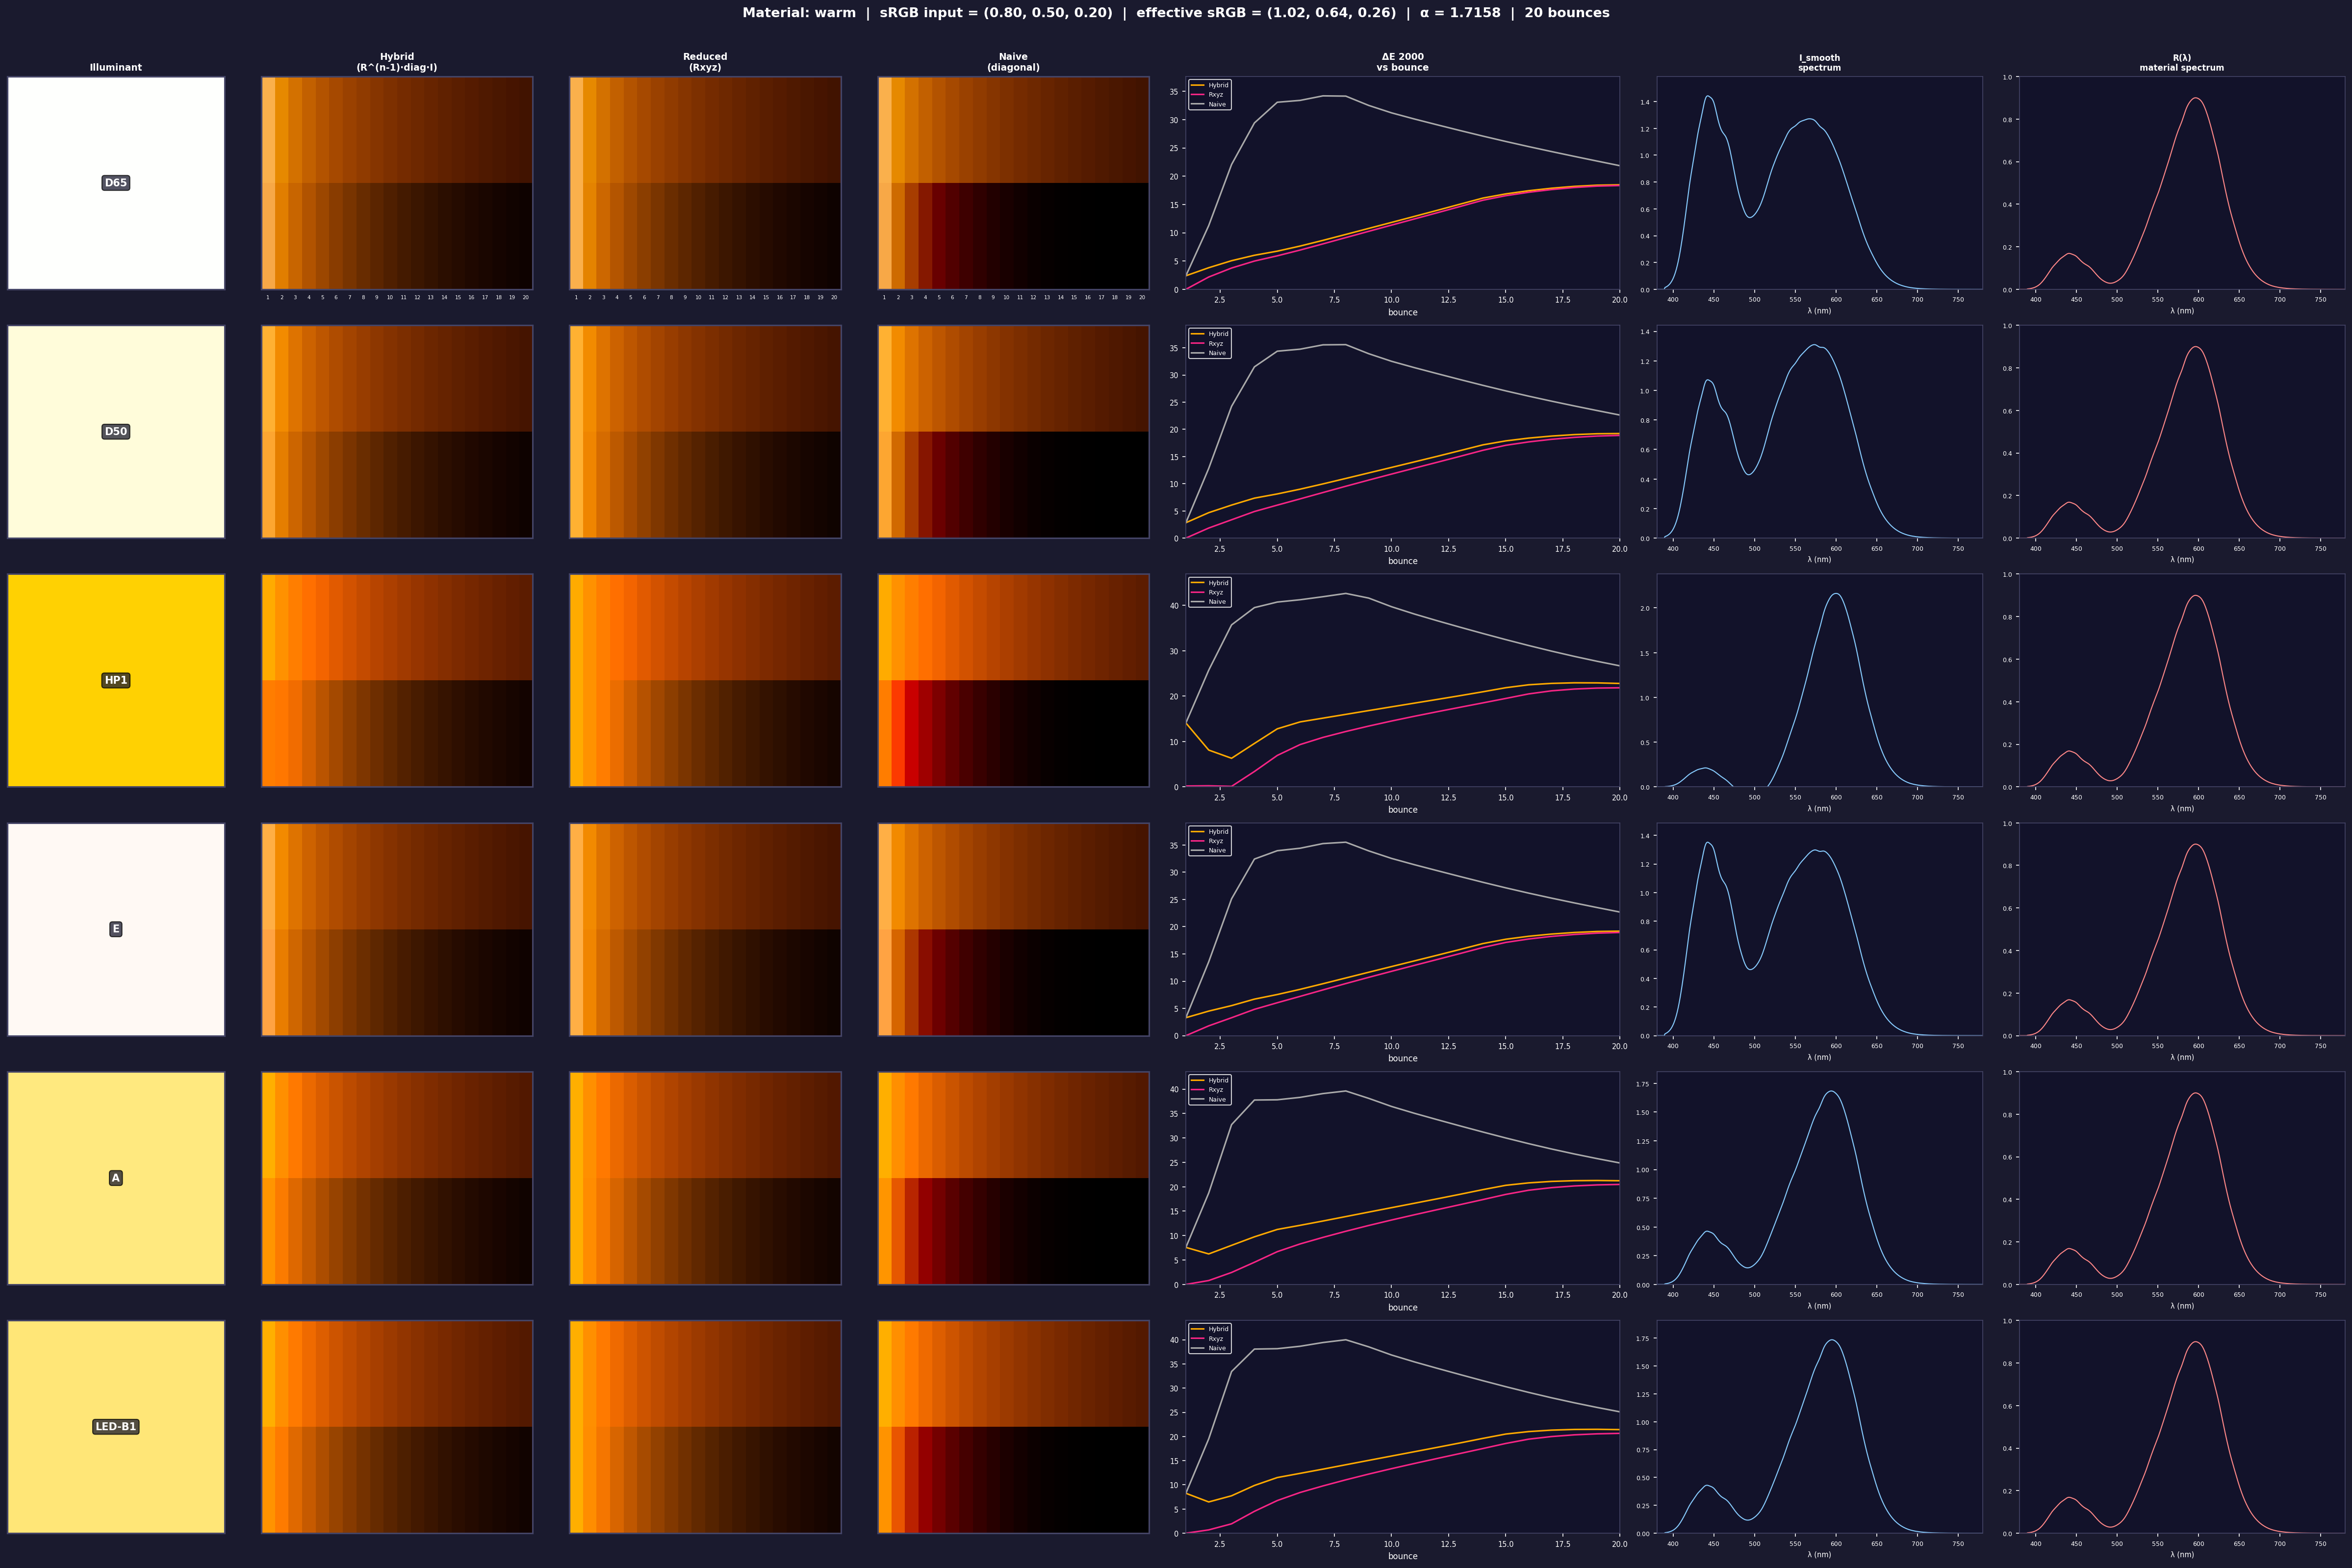
\includegraphics[width=\linewidth]{reflectance_warm.png}\\[1em]
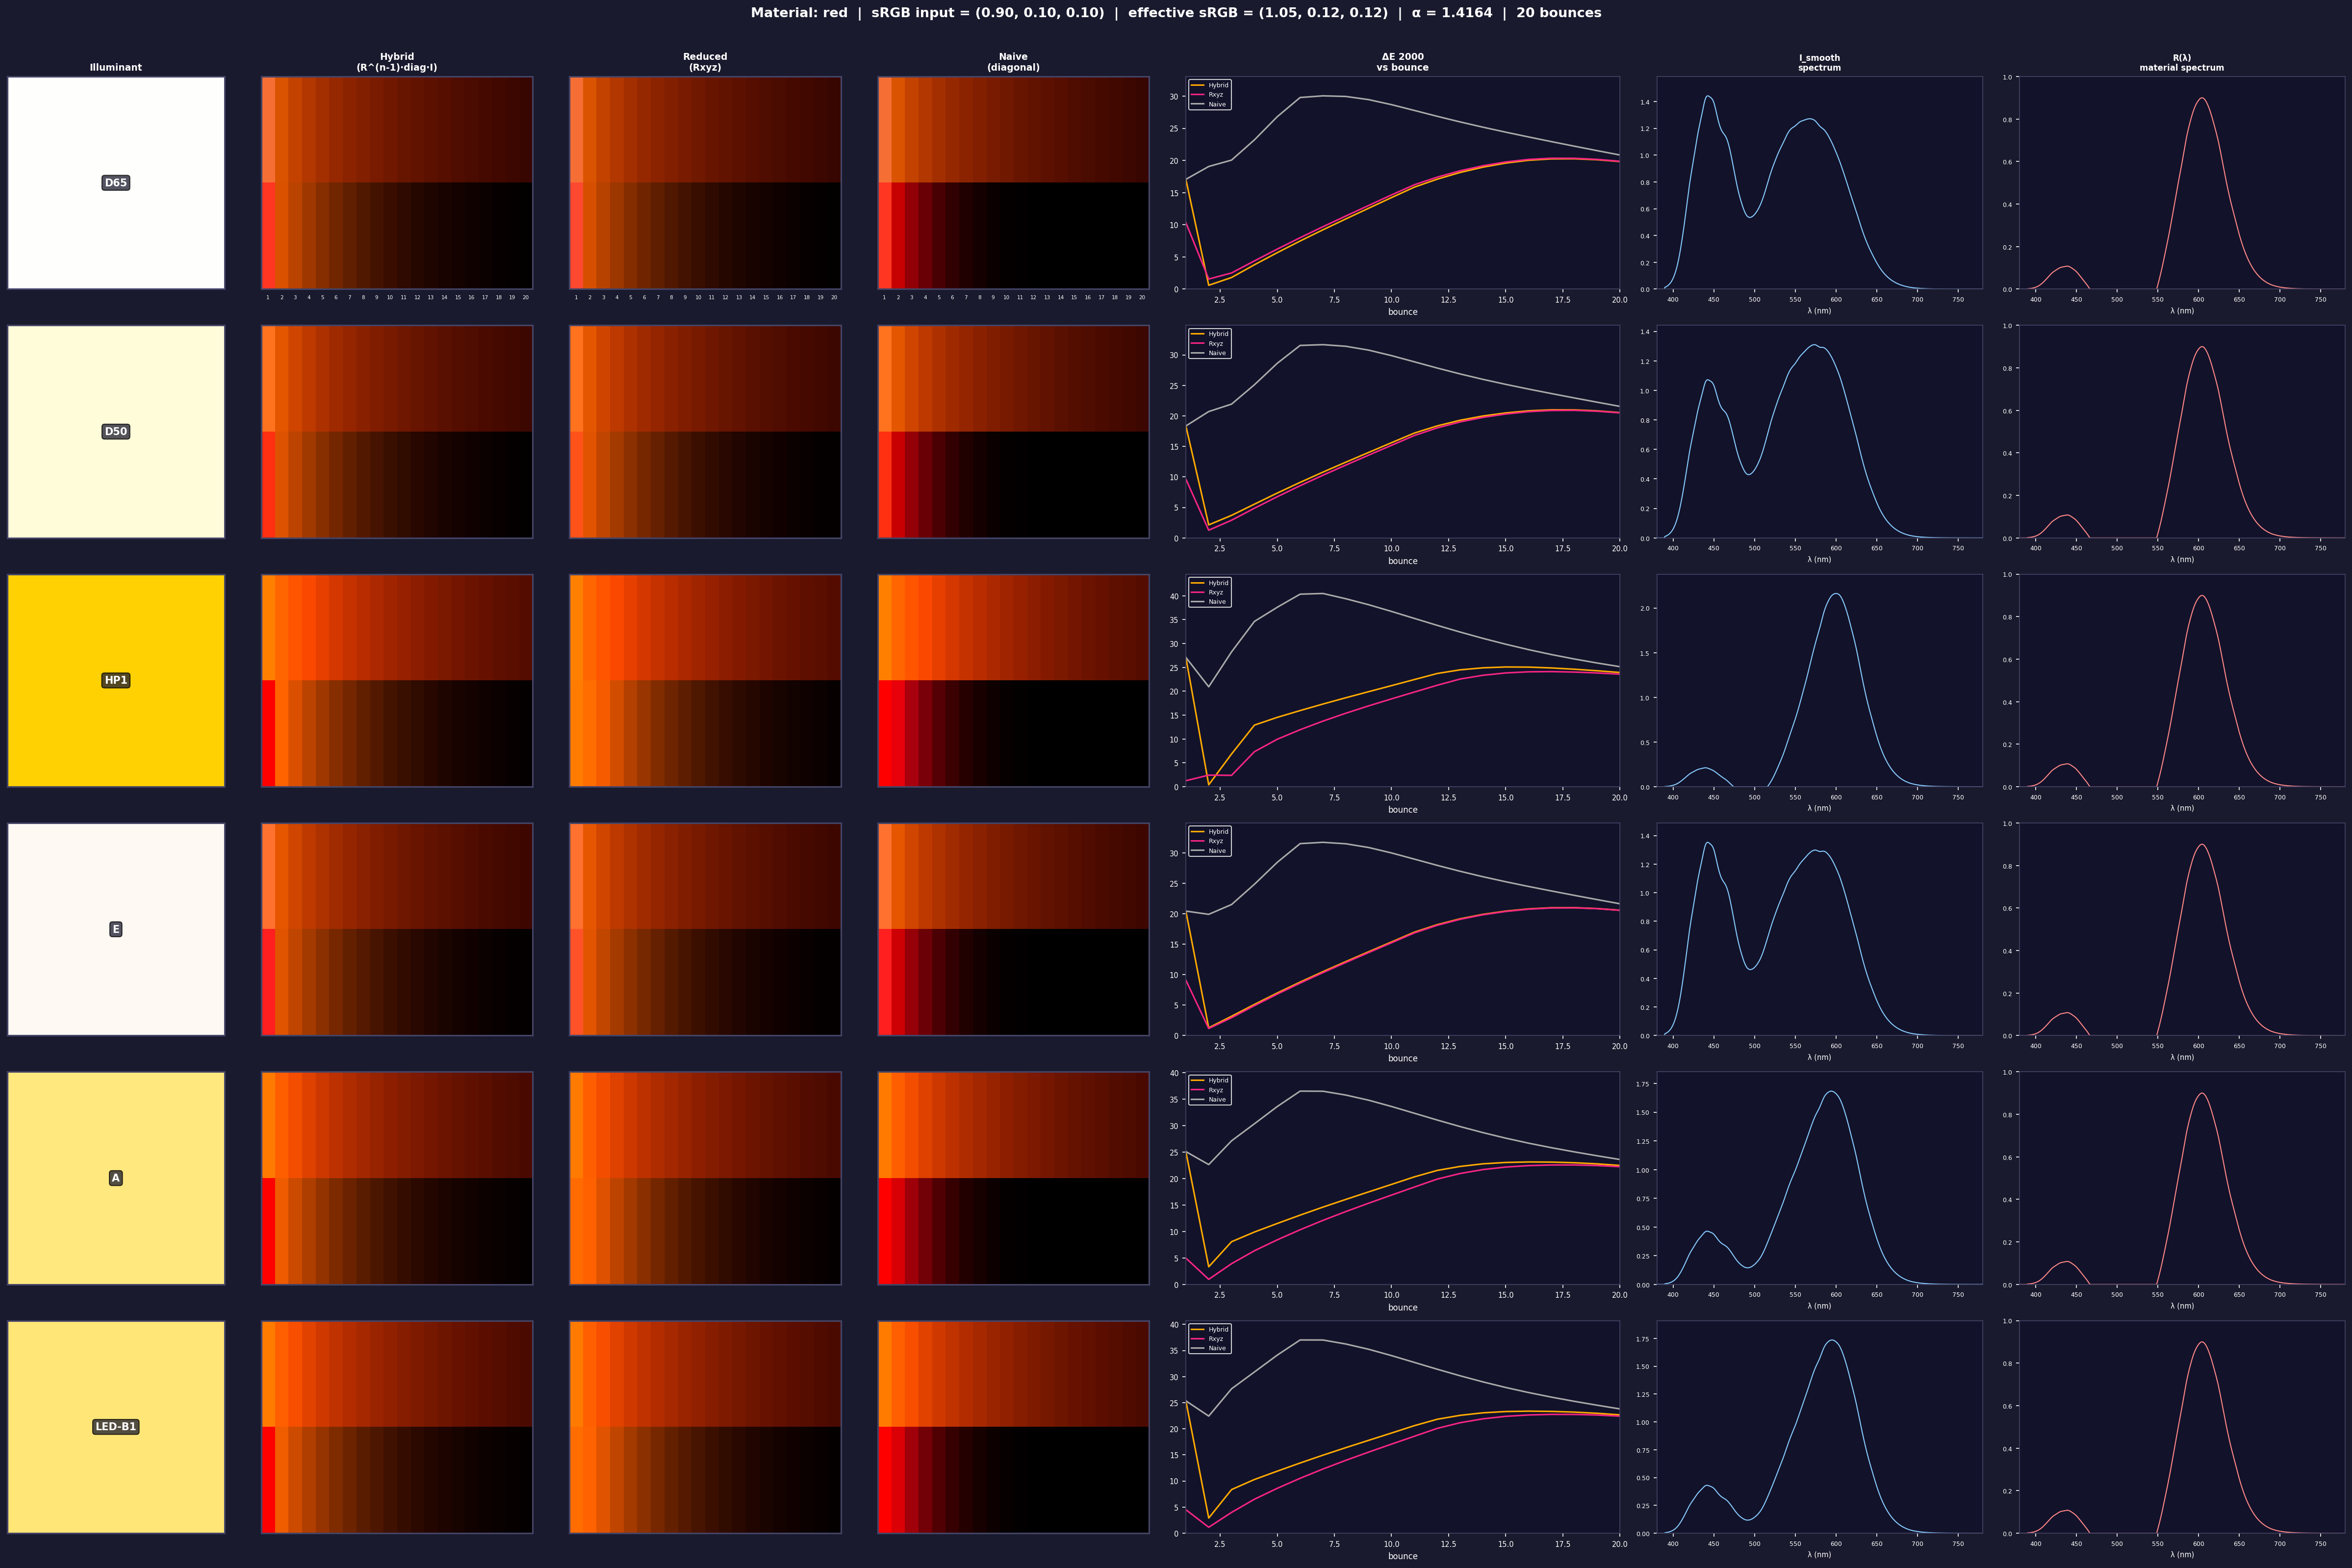
\includegraphics[width=\linewidth]{reflectance_red.png}
\caption{\file{validate\_reflectance.py}, materials \emph{warm} (top) and
\emph{red} (bottom).  Columns: illuminant, Hybrid, Reduced, Naive, $\dE$ vs
bounce, $\vL_{\text{smooth}}$, $\vr(\lambda)$.  The alpha scaling is visible in
the title (effective sRGB and $\alpha$).  The saturated red shows the regime
where the $\dE$ clipping convention matters (Section~\ref{sec:caveats}).}
\label{fig:refl}
\end{figure}

% ======================================================================
\section{Fluorescence}
\label{sec:fluo}

\subsection{Spectral model}

Fluorescence moves energy \emph{between} wavelengths: light absorbed at
$\lambda_i$ is re-emitted at $\lambda_o>\lambda_i$.  The reference builds the
reradiation matrix explicitly,
\begin{equation}
  \mF[\lambda_o,\lambda_i] = \bar\alpha\,a_{\max}\;
  e^{-\frac{(\lambda_i-\mu_a)^2}{2\sigma_a^2}}\;
  e^{-\frac{(\lambda_o-\mu_e)^2}{2\sigma_e^2}}\;
  \mathbb{1}[\lambda_o>\lambda_i],
  \qquad
  a_{\max} = \Big(\max_{\lambda_i}\sum_{\lambda_o}\mF[\lambda_o,\lambda_i]\Big)^{-1},
  \label{eq:Fspec}
\end{equation}
a separable absorption--emission Gaussian pair masked by the Stokes-shift
Heaviside, normalised so that the most absorbing wavelength re-emits at most
its full energy ($\bar\alpha\in[0,1]$ then scales the yield).  One complete
interaction is
\begin{equation}
  \mP = \diag(\vr) + \mF\,\diag(\mathbf 1-\vr),
  \label{eq:Pspec}
\end{equation}
which reads: the fraction $\vr$ is reflected at the same wavelength (diagonal),
the fraction $1-\vr$ is absorbed and a part of it re-emitted elsewhere
(off-diagonal).  This is the paper's $\mP = \mR + \mF(\mI-\mR)$ at full
spectral resolution, $500\times500$ here.

\subsection{Analytic Gaussian model (what the shader evaluates)}

Reducing Eq.~\eqref{eq:Pspec} gives $\mPb = \mRb + \mFb(\mI-\mRb)$ with
$\mFb = \mS\transp\mF\mSd$.  The brute-force $\mFb$ requires the
$500\times500$ matrix; the contribution of Belcour et al.\ (2025) is a
closed form that needs only the five Gaussian parameters.  The CMFs are first
approximated by $M=5$ one-dimensional Gaussians (the paper's Table~1),
$\mS \approx \mG\,\mTG$ with $\mG\in\mathbb{R}^{N\times5}$, and the
correction $\mC = \big((\mG\mTG)\transp(\mG\mTG)\big)^{-1}$ compensates for the
fit.  Products of Gaussians are Gaussians and their integral against the
Heaviside is an error function, so each entry of
$\mFc\in\mathbb{R}^{5\times5}$ has a closed form (paper Eq.~28) and
\begin{equation}
  \mFb_{\text{an}} = \mTG\transp\,\mFc\,\mTG\,\mC .
  \label{eq:Fan}
\end{equation}
The scripts compute both $\mFb_{\text{bf}}$ and $\mFb_{\text{an}}$ and print
their difference for every material.  Two implementation points:
\begin{itemize}[nosep]
  \item $\mTG$ is obtained by a \emph{dense least-squares fit}
        (\code{lstsq(G, S4)}), not by the paper's canonical 0/1 grouping
        (Eq.~29).  The grouping assumes the standard-scale CMFs the Gaussians
        were fitted to; our basis is column-normalised, so the dense fit is
        what reconstructs it.  Maximum fit error: $0.0090$.
  \item The effective yield is $\alpha = \bar\alpha\,\alpha_{\max}(\mu_e,\sigma_e)$
        with $\alpha_{\max}$ the conservative energy bound of paper Eq.~33.
\end{itemize}

\subsection{The U channel and the two albedo methods}
\label{sec:umethods}

The fourth channel $U$ is a UV Gaussian CMF.  The albedo's $U$ coordinate,
$\rho_U$, is needed to build $\mRb$ but is not available from an RGB colour.
It is computed in two ways:
\begin{align}
  \text{Method 1 (spectral):}   &\quad \rho_U = \vr\transp\,\mS_{:,U}, \\
  \text{Method 2 (projection):} &\quad \rho_U = \operatorname{clip}\!\big(\mathbf{t}_U\transp\vrho_{XYZ},\,0,1\big),
  \qquad \mathbf{t}_U = \mS_{:,U}\transp\,\mSd_{3},
\end{align}
where $\mSd_3$ is the dual of the XYZ sub-basis.  Method~1 needs the spectrum
and is the reference; Method~2 is a $3$-vector dot product (paper Eq.~31) and
is what a shader can do; it ships as \code{UV\_WEIGHTS}.  Every figure is
produced for both, and \file{u\_channel\_comparison.png}
(Figure~\ref{fig:uch}) plots the two $\rho_U$ across all materials.

\subsection{Six pipelines}

This table gives a summary of our experiment.  The reference is reduced
\emph{after} the last bounce; every model is reduced \emph{before} the first.

\begin{table}[h]\centering\small
\begin{tabular}{@{}lllll@{}}
\toprule
Pipeline & Operator & Light enters as & Dim.\ during transport & Reduced \\
\midrule
Spectral ref.  & $\mP$ (Eq.~\ref{eq:Pspec}) & $\vL_0$ & $N=500$ & after bounce $n$ \\
BF-reduced     & $\mPb_{\text{bf}} = \mRb+\mFb_{\text{bf}}(\mI-\mRb)$ & $\vc_0=\mS\transp\vL_0$ & $K=4$ & before \\
Analytic-red.  & $\mPb_{\text{an}} = \mRb+\mFb_{\text{an}}(\mI-\mRb)$ & $\vc_0$ & 4 & before \\
Hybrid         & $\mH=\mathbf D+\mFb_{\text{an}}(\mI-\mathbf D)$, then $\mPb_{\text{an}}$ & $\vc_0$ & 4 & before \\
Naive          & $\vrho^{\circ n}\circ\vc_0$ & $\vc_0$ & 4 & before \\
R-only ref.    & $\diag(\vr)$ (no $\mF$) & $\vL_0$ & 500 & after \\
\bottomrule
\end{tabular}
\caption{Bounce $n$ of a model is $\mPb^{\,n}\vc_0$ (Hybrid:
$\mPb_{\text{an}}^{\,n-1}\mH\vc_0$).  The R-only row is not a model: it is the
spectral reference with fluorescence switched off, and its $\dE$ against the
full reference measures how much of the signal \emph{is} fluorescence.}
\label{tab:pipelines}
\end{table}

The gap between BF-reduced and Analytic-reduced isolates one thing only, the
Gaussian-fit error of Eq.~\eqref{eq:Fan}; the gap between BF-reduced and the
spectral reference is the metameric-black error of the reduction itself.

\subsection{Display and metric}

The $U$ coordinate is dropped (paper Eq.~30), normalised XYZ is converted to
standard XYZ and then to linear sRGB with the IEC 61966-2-1 matrix, and the
swatches are gamma-encoded and clamped to $[0,1]$.  $\dE$ is computed from the
\emph{linear} sRGB values via CIELAB under D65, so the metric is a display-space
quantity rather than a distance in the normalised basis.

\subsection{Experiment and figures}

Eight materials, six illuminants, 20 bounces, both $U$ methods, with
$\bar\alpha=0.95$, $\mu_a=380$\,nm (UV absorption, to exercise the $U$
channel), $\mu_e=520$\,nm, $\sigma_a=30$, $\sigma_e=20$.  Per material and
method the script writes the main panel (Figure~\ref{fig:fluo}) and a
diagnostic sheet (Figure~\ref{fig:diag}): chromaticity trajectory, luminance
and $U$ over bounces, and the spectra with and without fluorescence with the
$\bar u$ CMF overlaid.  For two representative materials it also sweeps
$(\mu_a,\mu_e)$ (Figure~\ref{fig:sweep}) and $(\sigma_a,\sigma_e)$, and a
separate panel compares D65 with a pure-UV Gaussian illuminant.

\begin{figure}[p]\centering
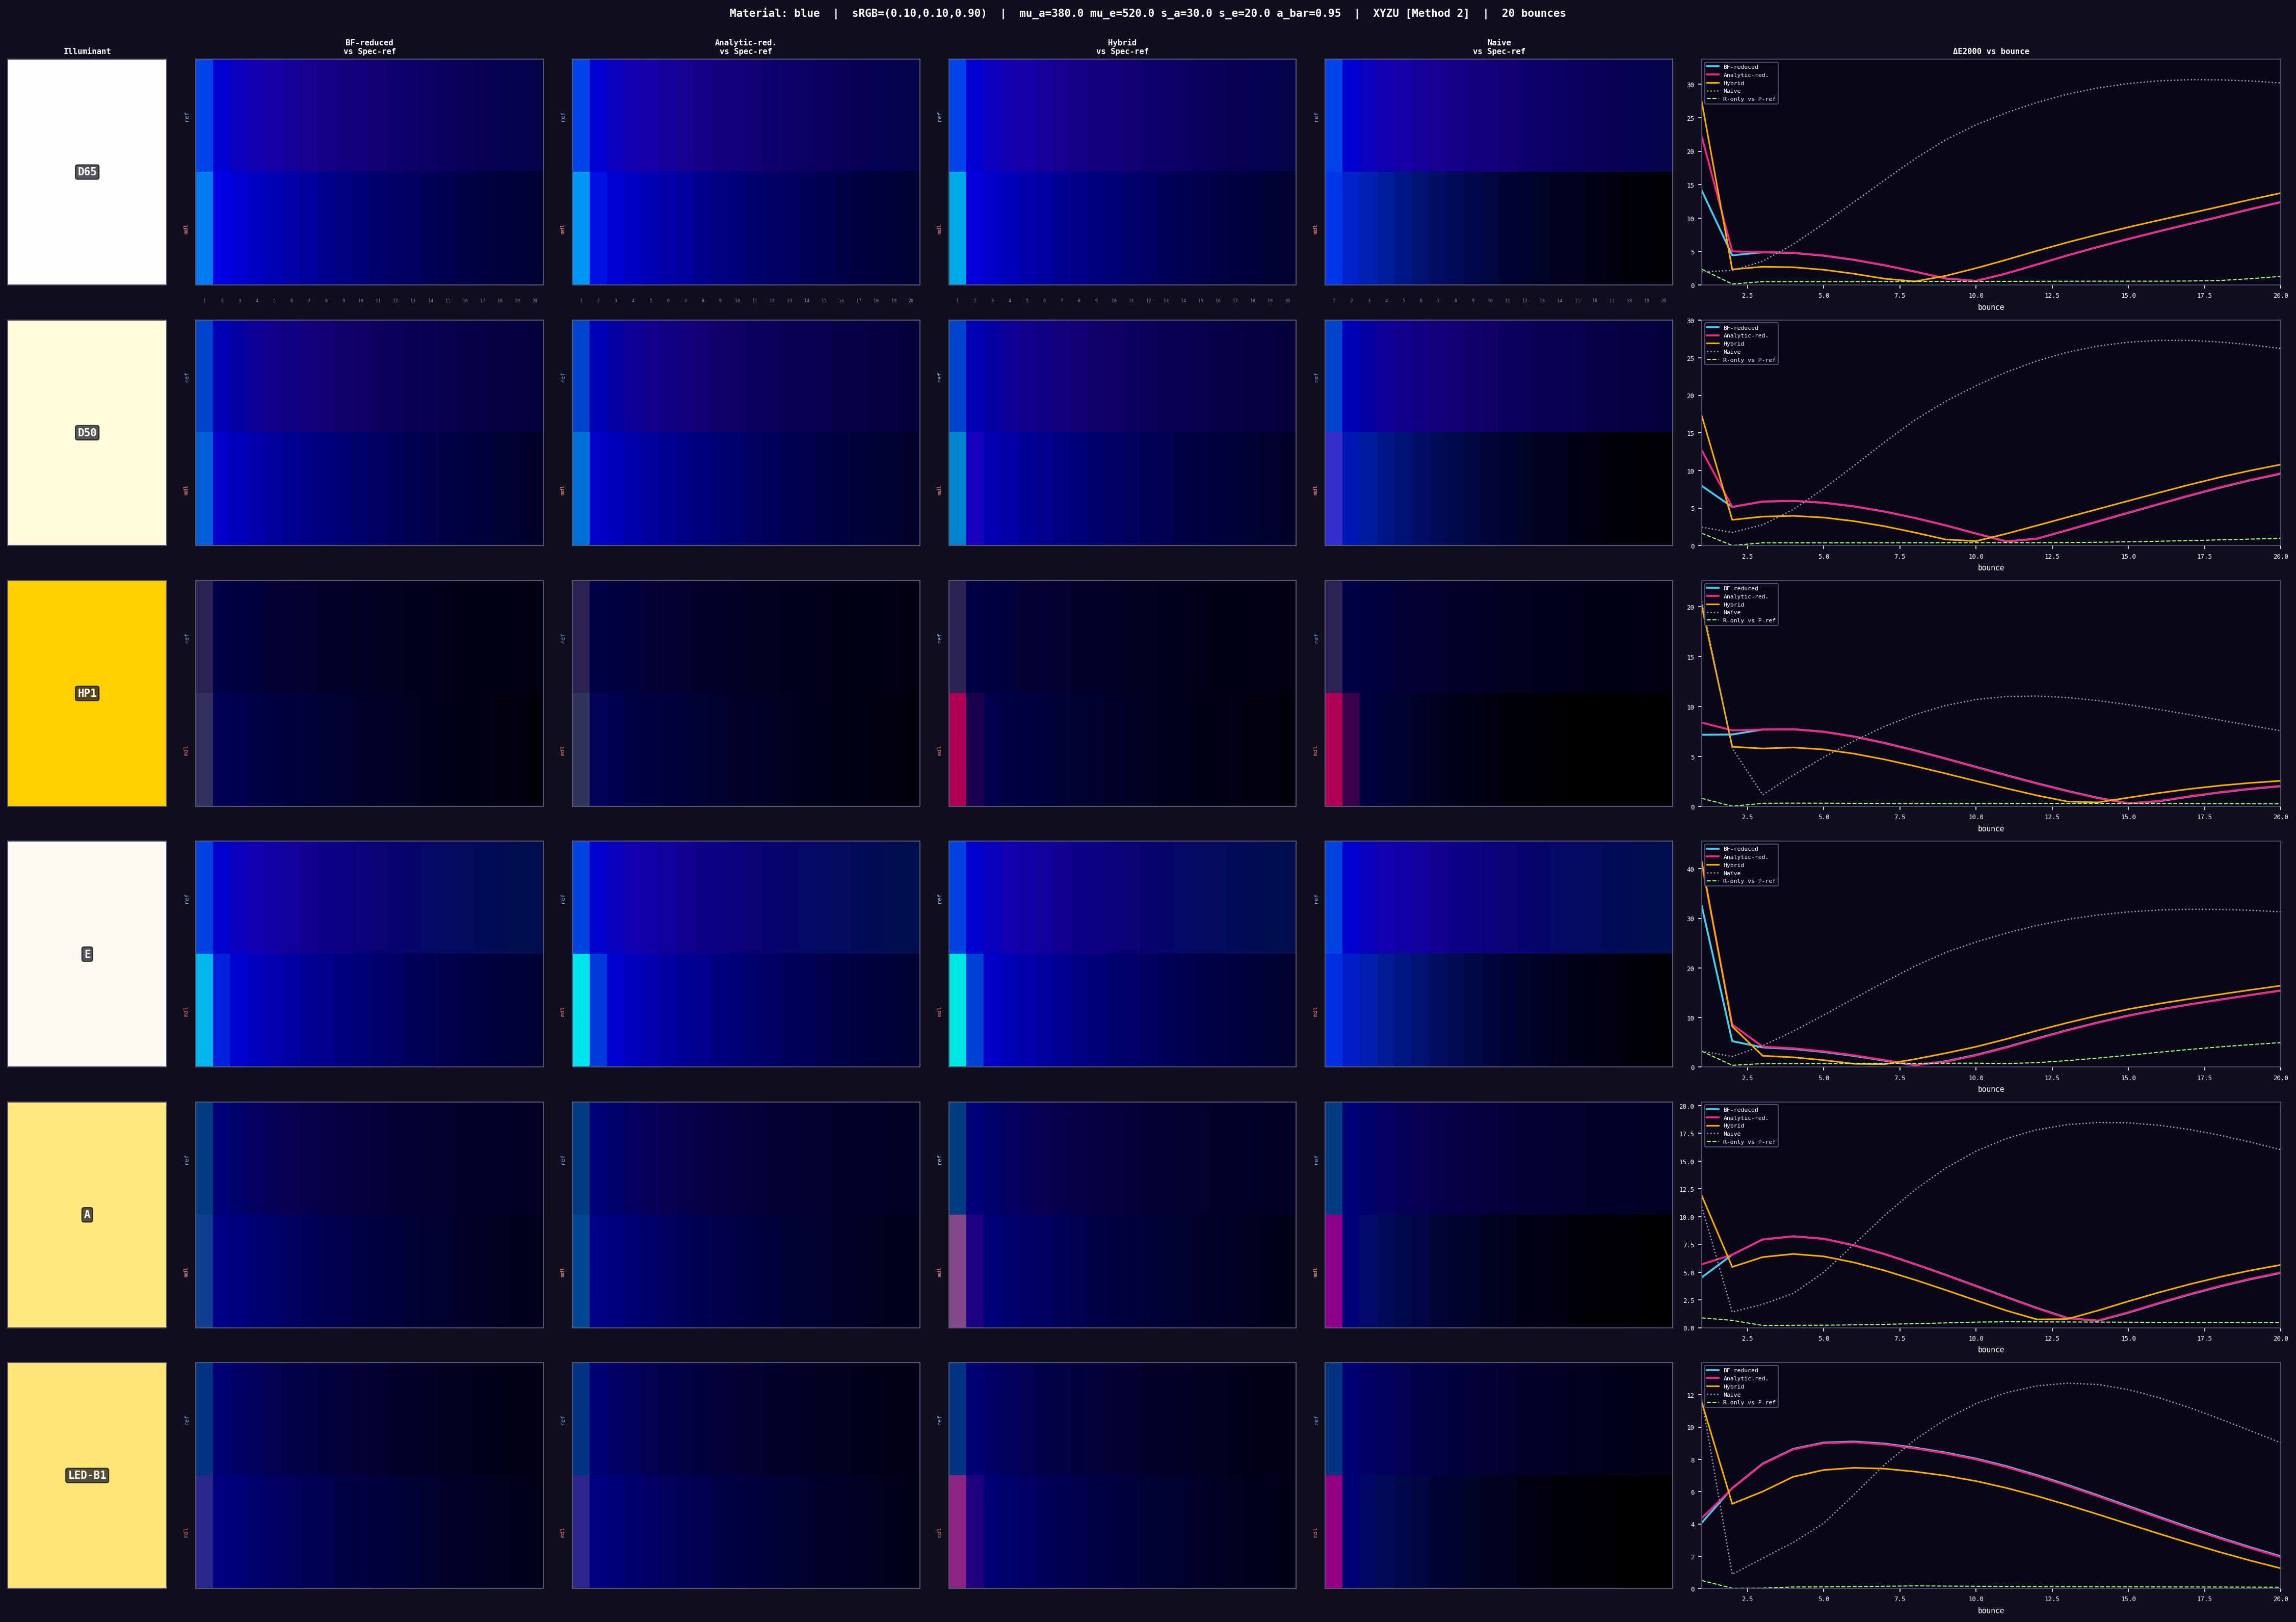
\includegraphics[width=\linewidth]{fluorescence_m2_blue.png}
\caption{\file{validate\_fluorescence.py}, material \emph{blue}, Method~2.
Columns: illuminant, BF-reduced, Analytic-reduced, Hybrid, Naive, $\dE$ vs
bounce.  Each swatch: reference above, model below, bounces left to right.}
\label{fig:fluo}
\end{figure}

\begin{figure}[p]\centering
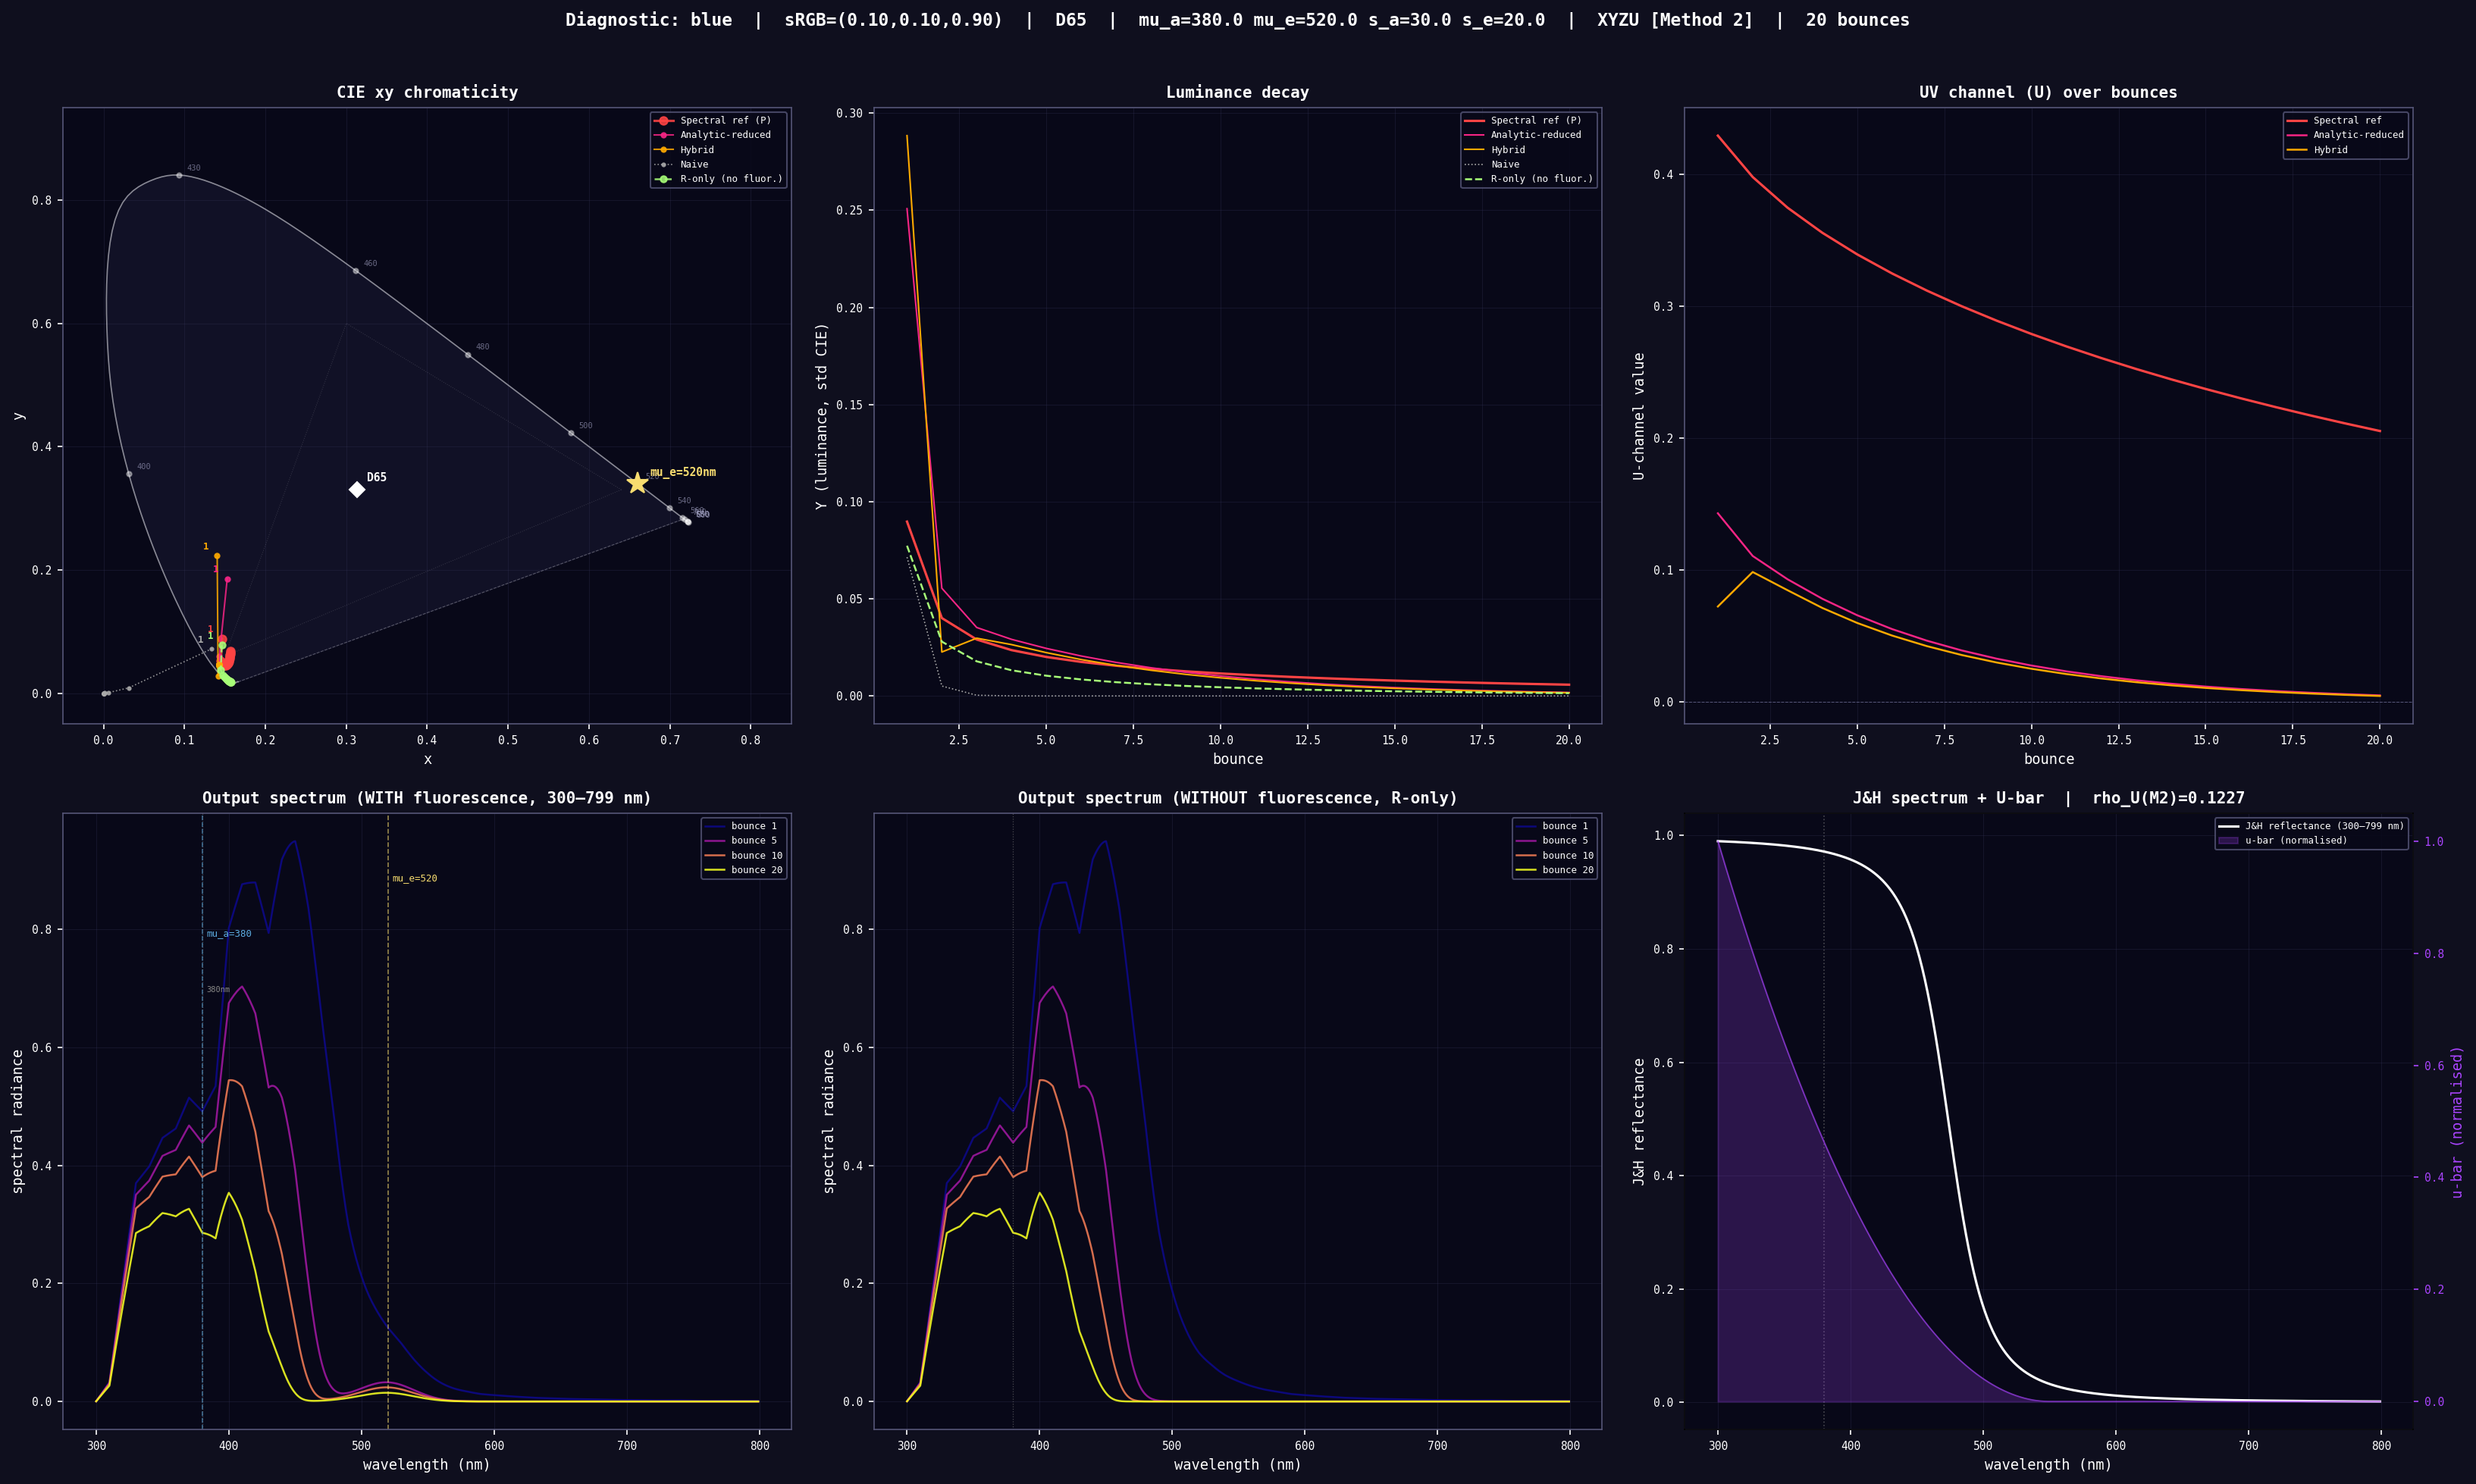
\includegraphics[width=\linewidth]{fluorescence_m2_blue_diag.png}
\caption{Diagnostics for the same material under D65: CIE $xy$ trajectory,
luminance and $U$ against bounce, spectra with and without fluorescence, and
the Jakob--Hanika albedo with the $\bar u$ function overlaid.}
\label{fig:diag}
\end{figure}

\begin{figure}[t]\centering
\begin{minipage}[t]{0.48\linewidth}\centering
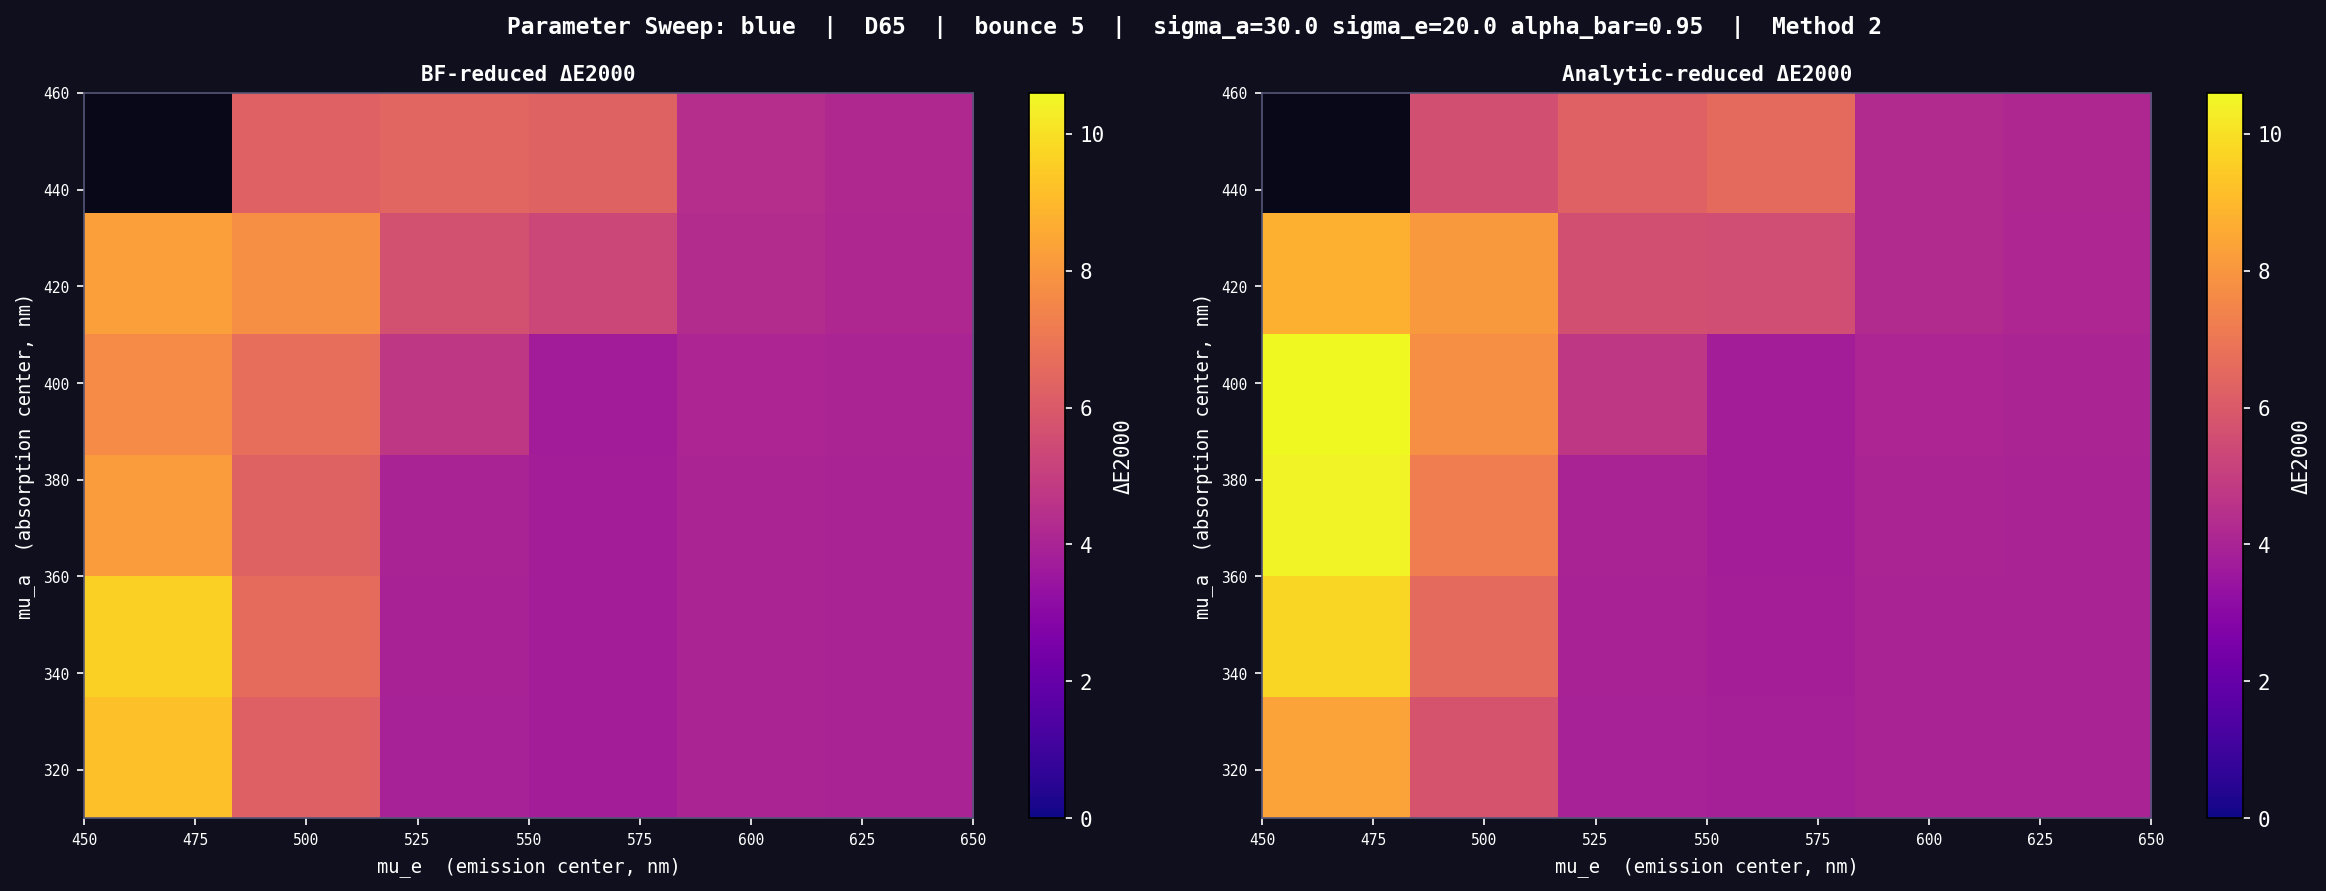
\includegraphics[width=\linewidth]{fluorescence_m2_blue_param_sweep.png}
\caption{$\dE$ at bounce 5 over the $(\mu_a,\mu_e)$ plane, material
\emph{blue}, Method~2.}
\label{fig:sweep}
\end{minipage}\hfill
\begin{minipage}[t]{0.48\linewidth}\centering
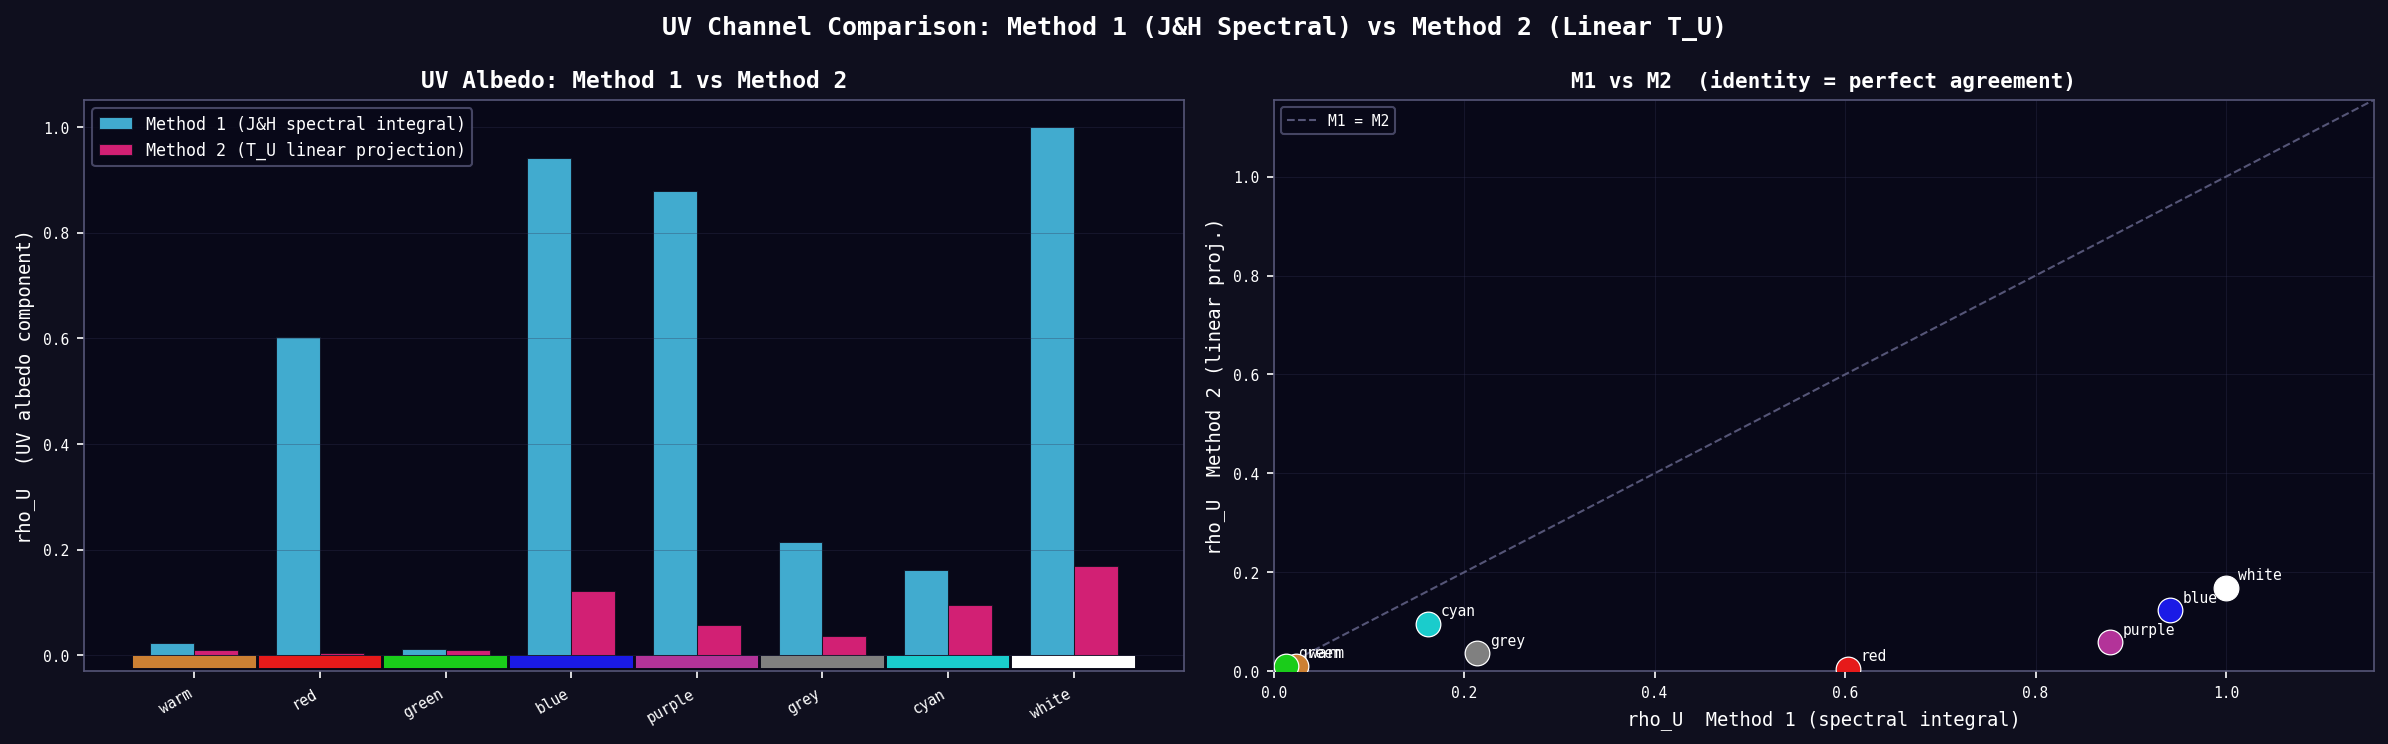
\includegraphics[width=\linewidth]{fluorescence_u_channel.png}
\caption{$\rho_U$ from the spectral integral (Method~1) and from the linear
projection (Method~2) across the eight materials.}
\label{fig:uch}
\end{minipage}
\end{figure}

% ======================================================================
\section{Diagonal versus reduced transport, the authors' figure}
\label{sec:upscale}

\file{fig\_upscale\_diag.py} reproduces a supplementary figure supplied by
Laurent Belcour, with the authors' private modules replaced by numpy and
matplotlib.  Eight XYZ inputs are projected to valid spectra ($\mSd\vc$, scaled
to a peak of $0.8$, clipped), then transported for ten bounces both
diagonally and through $\mRb$; the script plots $\dE$ in $xy$, in $Y$ and in
XYZ against bounce, the chromaticity trajectory on the spectral locus, and the
reconstructed spectra (Figure~\ref{fig:upscale}).  Aligning our pipeline on
this script fixed three conventions that the rest of the repository inherits:
column-normalised CMFs with no extra $\sum\bar y$ factor, no chromatic
adaptation, and the naive baseline defined as a component-wise power in XYZ.

\begin{figure}[h]\centering
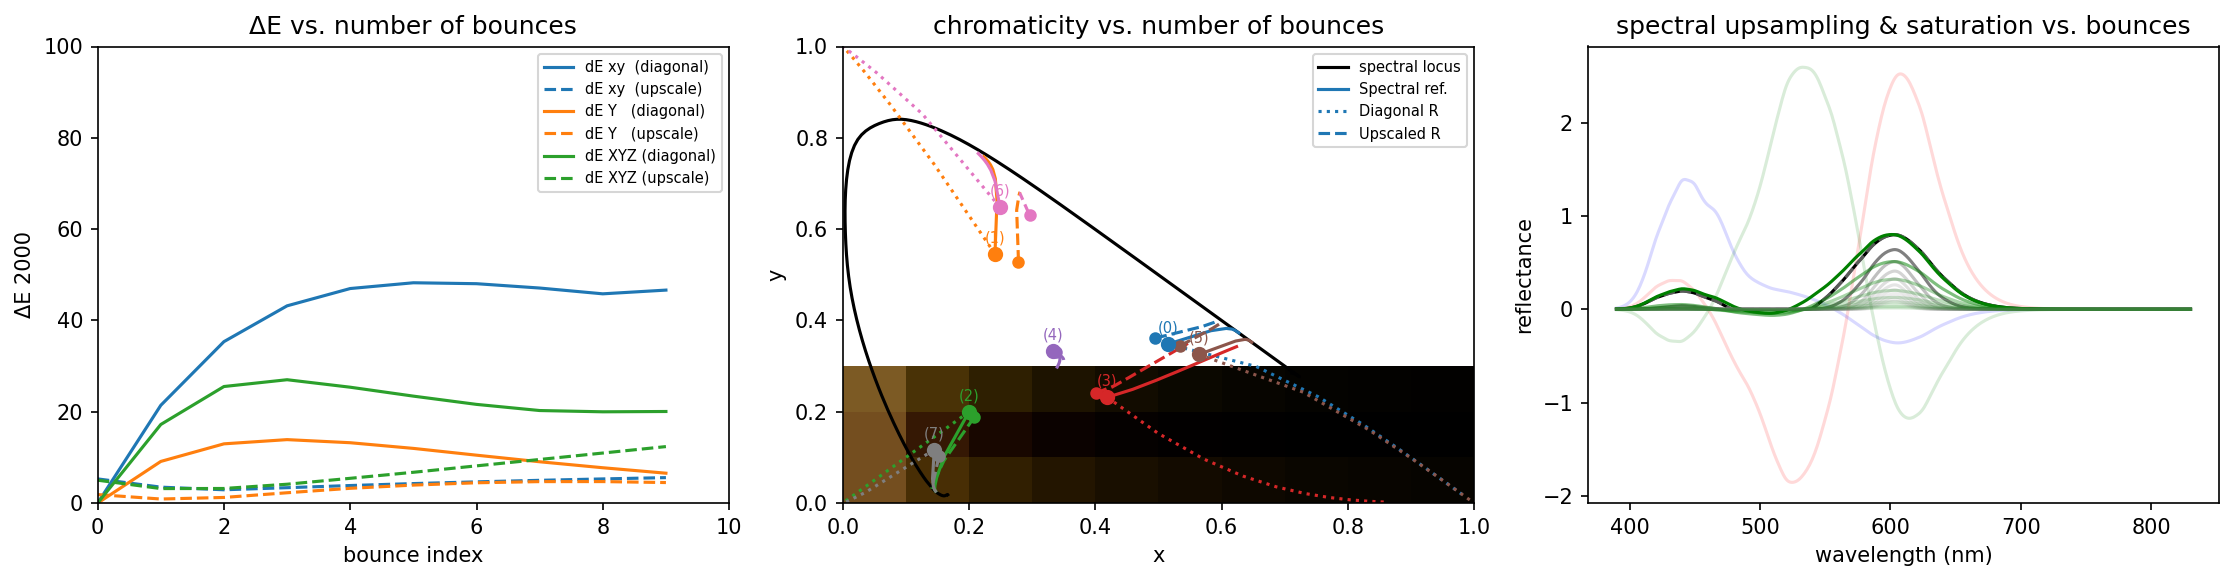
\includegraphics[width=\linewidth]{upscale_de_chroma_spectra.png}
\caption{\file{fig\_upscale\_diag.py}: $\dE$ vs bounce for diagonal and reduced
transport (left), chromaticity drift over bounces (centre), spectral
reconstruction and saturation (right).}
\label{fig:upscale}
\end{figure}

% ======================================================================
\clearpage
\section{Bridge to the Godot implementation}
\label{sec:godot}

\subsection{Emitted constants and their layout}

\file{generate\_godot\_matrices.py} rebuilds the XYZU basis exactly as
\file{validate\_fluorescence.py} does, derives every fixed matrix, runs the
self-checks of Table~\ref{tab:selfchecks}, and prints the literals to paste
into the addon.  Layout matters because GLSL matrices are column-major while
the Python side is row-major:

\begin{table}[h]\centering\small
\begin{tabular}{@{}llll@{}}
\toprule
Constant & Shape & Emitted as & Consumer \\
\midrule
\code{Rx, Ry, Rz, Ru} (Eq.~\ref{eq:Rk}) & $4\times4$ & GLSL \code{mat4}, each \code{vec4} one \emph{column} & shader \\
\code{C} & $4\times4$ & row-major \code{float[16]} & shader \\
\code{UV\_WEIGHTS} $=\mathbf t_U$ & 3 & \code{vec3} & shader \\
\code{LIN\_SRGB\_TO\_NORM\_XYZ}, inverse & $3\times3$ & row-major \code{float[9]} & shader \\
\code{TG\_T} ($4\times5$), \code{TG} ($5\times4$), \code{C\_MAT} & -- & GDScript \code{Array[float]}, row-major & controller \\
\bottomrule
\end{tabular}
\caption{The controller computes $\mFb$ on the CPU from Eq.~\eqref{eq:Fan}
whenever a Gaussian parameter changes and uploads it as a \code{mat4}; the
shader evaluates $\mRb\vc + \mFb\big((\mI-\mRb)\vc\big)$ per fragment.}
\label{tab:layout}
\end{table}

\begin{table}[h]\centering\small
\begin{tabular}{@{}lr@{}}
\toprule
Self-check & Value \\
\midrule
$\max|\mS_4\transp\mSd_4-\mI_4|$ & $3.8\times10^{-15}$ \\
$\max|\mS_3\transp\mSd_3-\mI_3|$ & $9.7\times10^{-16}$ \\
Gaussian CMF fit, $\max|\mS_4-\mG\mTG|$ & $0.0090$ \\
$\max|\mC-\mC\transp|$ & $2.8\times10^{-13}$ \\
$\max|\sum_k\mR_k-\mI_4|$ (intrinsic reduction error of a flat spectrum) & $0.108$ \\
$\max|\code{LIN\_TO\_NORM}\cdot\code{NORM\_TO\_LIN}-\mI_3|$ & $1.4\times10^{-7}$ \\
\bottomrule
\end{tabular}
\caption{Printed by \file{generate\_godot\_matrices.py}.  The last line is the
rounding of the two published sRGB matrices, not a defect.  The
$\sum_k\mR_k$ line is informational: a flat spectrum is not in the span of
$\mSd_4$, so its reduced reflectance is not exactly the identity.}
\label{tab:selfchecks}
\end{table}

\subsection{What the shader does with the albedo}
\label{sec:shader-albedo}

For the record, and because it differs from the reflectance script's treatment,
the direct-lighting shader builds its 4-D albedo as
\begin{verbatim}
vec3  albedo_linear = texture(albedo, UV).rgb;
vec3  albedo_xyz    = LIN_SRGB_TO_NORM_XYZ * albedo_linear;
float albedo_u      = clamp(dot(albedo_xyz, UV_WEIGHTS), 0.0, 1.0);
vec4  rho           = vec4(albedo_xyz, albedo_u);
\end{verbatim}
So Method~2 is what the engine uses: $\rho_U$ comes from the linear projection
$\mathbf t_U$ of Section~\ref{sec:umethods}, which is why that method is
validated next to the spectral integral rather than only mentioned.  Only
$\rho_U$ is clamped; the XYZ coordinates are used as they come out of the
texture conversion.  No alpha scaling is applied: the reconstructed
reflectance spectrum implied by a
saturated authored colour can therefore exceed unity in the engine, which is
exactly the regime Section~\ref{sec:alpha} identifies as unphysical.  Under
direct lighting alone the consequence is bounded, but it is the first thing to
revisit if the shader is extended to multiple bounces, where
Figure~\ref{fig:refl} shows the error compounding.

\subsection{Verification against the Python reference}

The following scripts compare the engine's algebra with the validated pipeline
and exit non-zero if a check fails, so they also serve as regression tests.

\paragraph{\file{verify\_fbar\_convention.py}} builds, for one test material
($\mu_a=430$, $\sigma_a=40$, $\mu_e=560$, $\sigma_e=40$, $\bar\alpha=0.8$),
the brute-force $\mFb_{\text{bf}}$, the validated $\mFb_{\text{an}}$, and the
controller's $\mFb$ under two conventions: the one first written, and the
corrected one.  Comparing the \emph{effective} operator each applies to a
colour is what exposed two bugs in the original controller:
\begin{enumerate}[nosep]
  \item the $\mFc$ indices were swapped (absorption paired with the emission
        Gaussian index and vice versa, against paper Eq.~16);
  \item the $4\times4$ was uploaded as a \code{Projection} whose columns were
        the rows of $\mFb$, so the shader applied $\mFb\transp$.
\end{enumerate}

\paragraph{\file{verify\_godot\_shader.py}} takes an arbitrary 4-D albedo and
4-D light and checks that the shader's factored evaluation reproduces
$(\mRb+\mFb(\mI-\mRb))\vc$ for both the reduced and the diagonal reflectance,
since the shader exposes both.

\begin{table}[h]\centering\small
\begin{tabular}{@{}llr@{}}
\toprule
Script & Check & Value \\
\midrule
\file{verify\_fbar\_convention} & corrected controller $\mFb$ vs $\mFb_{\text{an}}$ & $8.0\times10^{-17}$ \\
                                & original effective operator vs $\mFb_{\text{an}}$ & $0.53$ \\
                                & $\|\mFb_{\text{an}}-\mFb_{\text{bf}}\|_F$ (model approximation) & $0.168$ \\
\file{verify\_godot\_shader}    & controller $\mFb$ vs validated & $7.0\times10^{-17}$ \\
                                & shader output, reduced $\mRb$ & $1.2\times10^{-16}$ \\
                                & shader output, diagonal $\mathbf D$ & $1.1\times10^{-16}$ \\
\bottomrule
\end{tabular}
\caption{Current values (\code{make check}).  Everything that should be zero
is at double precision; the $0.53$ line documents that the pre-fix convention
was wrong by a large margin, not by a rounding artefact.  The $0.168$ line is
the closed-form Gaussian model's approximation of the true reradiation matrix
for this material; the $\dE$ curves of Section~\ref{sec:fluo} measure its
perceptual effect, and it is guarded here only against regression.}
\label{tab:checks}
\end{table}

% ======================================================================
\section{Consistency notes and caveats}
\label{sec:caveats}

The following points are choices, not bugs, but they affect how the numbers
should be read.

\begin{enumerate}
  \item \textbf{Two different bases} (Table~\ref{tab:bases}).  The reflectance
        and fluorescence scripts do not share a grid, a CMF set or a value of
        $K$.  Albedo coordinates and $\dE$ values are not comparable between
        them.
  \item \textbf{Two different $\dE$ clipping conventions.}
        \file{validate\_fluorescence.py} clips linear sRGB at $0$ only before
        computing $\dE$; \file{validate\_reflectance.py} clips to $[0,1]$.  In the
        latter, once both reference and model exceed the display range they
        both clip to white and the reported $\dE$ collapses, so the curves are
        optimistic in the saturated regime (visible in Figure~\ref{fig:refl},
        bottom).  The swatches, clamped in both scripts, do not show the
        difference.
  \item \textbf{Two XYZ conventions in the reflectance script.}
        \file{validate\_reflectance.py} reconstructs its spectrum from standard
        CIE XYZ but projects and reduces with the column-normalised basis.  The
        round trip is exact (it is checked), so the script is self-consistent,
        but its $\vrho$ is on a different scale from the normalised-XYZ
        convention of the fluorescence script.
  \item \textbf{Jakob--Hanika below 380\,nm} is an extrapolation of a fit made on
        the visible range.  The default $\mu_a=380$\,nm sits on that boundary.
        Results in the UV are therefore ``plausible'', not ``measured''.
  \item \textbf{$\mTG$ by dense least squares} rather than the paper's 0/1
        grouping, for the normalisation reason given in
        Section~\ref{sec:fluo}.
  \item \textbf{One constant corrected on conversion.}  The notebook from which
        \file{validate\_reflectance.py} was extracted had the XYZ$\to$sRGB entry
        $(3,1)$ as $0.0555434$; it is $0.0556434$ (IEC 61966-2-1) and was
        corrected.  The effect is below display precision.
  \item \textbf{Alpha scaling is validated but not ported.}  The engine applies
        neither upsampling variant to authored albedos
        (Section~\ref{sec:shader-albedo}); it consumes the albedo texture
        directly.  This is a known gap, not an oversight in the validation.
  \item \textbf{Analytic-model error is material-dependent.}  The $0.168$ of
        Table~\ref{tab:checks} is for one test material; the parameter sweeps
        (Figure~\ref{fig:sweep}) map how it varies with the absorption and
        emission positions.
\end{enumerate}

% ======================================================================
\section{Reproduction}
\label{sec:repro}

\begin{verbatim}
make venv            # python3 -m venv .venv ; pip install -r requirements.txt
make check           # verify_fbar_convention + verify_godot_shader, exit 1 on failure
make reflectance     # results/reflectance/        (~1 min)
make fluorescence    # results/fluorescence/       (several minutes)
make upscale         # results/upscale_diag/       (~10 s)
make matrices        # print the GLSL / GDScript constants
make doc             # this document (latexmk), after `make figures`
\end{verbatim}

All scripts resolve \file{data/} and \file{results/} relative to their own
location (\file{scripts/\_paths.py}) and can be run from any directory.  Pinned
versions: Python 3.12, numpy 2.4.6, scipy 1.17.1, matplotlib 3.10.9,
colour-science 0.4.7.  Every figure in \file{results/} is committed and was
produced with these versions.

% ======================================================================
\appendix
\section{File map}

\begin{table}[h]\centering\small
\begin{tabular}{@{}lp{9.2cm}@{}}
\toprule
Path & Role \\
\midrule
\file{scripts/validate\_reflectance.py}   & Section~\ref{sec:reflectance}; alpha scaling, Hybrid, smoothed illuminant \\
\file{scripts/validate\_fluorescence.py}  & Section~\ref{sec:fluo}; six pipelines, two $\rho_U$ methods, sweeps \\
\file{scripts/fig\_upscale\_diag.py}      & Section~\ref{sec:upscale}; authors' figure, standalone \\
\file{scripts/generate\_godot\_matrices.py} & Section~\ref{sec:godot}; emits engine constants with self-checks \\
\file{scripts/verify\_fbar\_convention.py} & Section~\ref{sec:godot}; controller $\mFb$ check, documents the two bugs \\
\file{scripts/verify\_godot\_shader.py}   & Section~\ref{sec:godot}; end-to-end shader algebra check \\
\file{scripts/\_paths.py}                 & repository-relative paths \\
\file{data/cmf/xyzu.csv}                  & XYZU CMFs, 300--799\,nm (Fichet et al.\ 2024 companion) \\
\file{data/cmf/ciexyz06\_2deg.csv}        & CIE 2006 $2^\circ$ XYZ (Belcour et al.\ 2025 supplement) \\
\file{data/srgb.coeff}                    & Jakob--Hanika sRGB coefficient table \\
\file{results/}                           & committed figures, one folder per script \\
\bottomrule
\end{tabular}
\end{table}

\section*{References}
\begin{itemize}[nosep]
  \item L.~Belcour, A.~Fichet, P.~Barla. \emph{A Fluorescent Material Model for
        Non-Spectral Editing \& Rendering.} SIGGRAPH 2025. hal-05267431.
  \item A.~Fichet, L.~Belcour, P.~Barla. \emph{Non-Orthogonal Reduction for
        Rendering Fluorescent Materials in Non-Spectral Engines.} Computer
        Graphics Forum, 2024.
  \item W.~Jakob, J.~Hanika. \emph{A Low-Dimensional Function Space for Efficient
        Spectral Upsampling.} Computer Graphics Forum (Eurographics), 2019.
\end{itemize}

\end{document}
